\section{Natural Language Generation}

Natural Language Generation (NLG) is a sub-field of Natural Language Processing that attempts to generate a sequence of words that resemble natural human languages. Traditionally, this can be done by either using production rules of a pre-defined grammar, or by performing statistical analyses of existing human-written texts to predict sequences of words based on their occurrence probabilities.

\section{Recurrent Neural Networks}

Recurrent neural networks (RNNs) are a sub-class of artificial neural networks that can be considered a neural network equivalent to a Hidden Markov Model. Its units forms a directed graph that operates on a sequence of inputs when unrolled temporally. This makes them useful to extract features from arbitrary length sequences of input like audio or text. The features extracted at a given temporal point in an instance (sequence) is given by the below equation. The language model is built in such a way that the features extracted from the sequence at epoch $t$ depend on the features observed during the epochs $0 \cdots t-1$

\begin{equation}
	P(w_1, \cdots, w_T) = \prod_{i=1}^T P(w_i | w_1, \cdots, w_{i−1})
\end{equation}

A graphical depiction of an unrolled RNN is shown in figure \ref{fig:recurrent-neural-network-unfold}

\begin{figure}[ht]
	\centering
	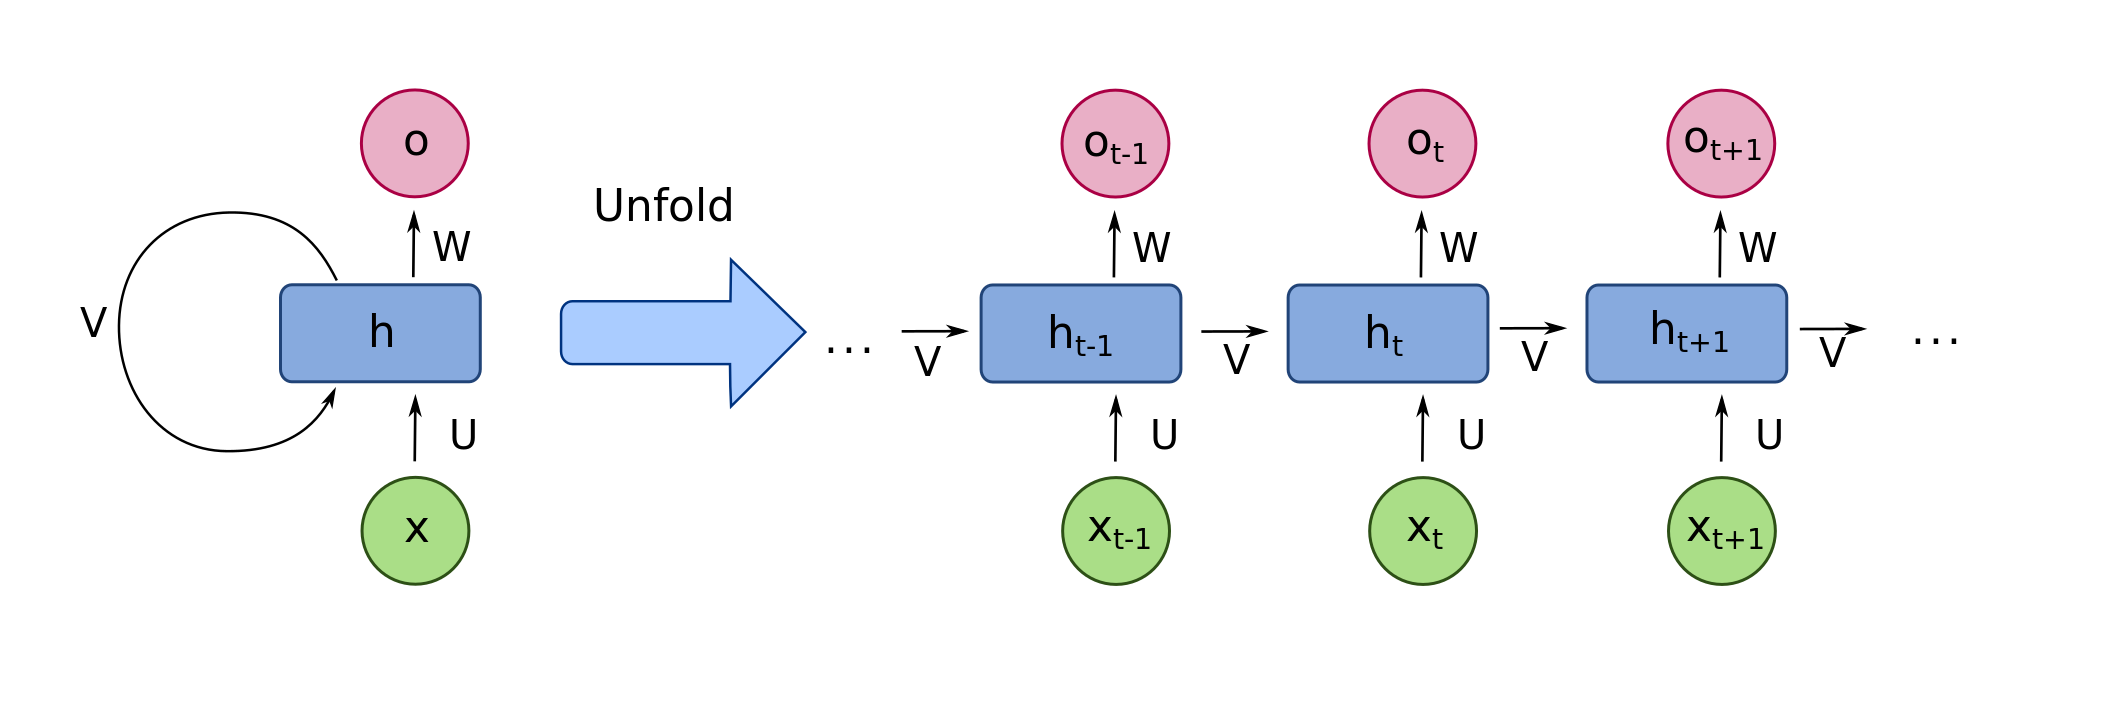
\includegraphics[width=.8\textwidth]{images/recurrent-neural-network-unfold}
	\caption{\label{fig:recurrent-neural-network-unfold} Unrolled RNN}
\end{figure}

The most recent and useful variants of recurrent units provide the ability to retain 'memory' of the context in which the current features are to be considered. In the domain of language processing, this typically implies that the recurrent unit has a stored memory of the previous seen words in a sequence, and this property grants it the ability to learn context as part of the feature space.

The prominent variants of recurrent units used in neural networks to extract features from sequences using a memory mechanism are Long Short-Term Memory (LSTM) units \cite{gers2001lstm} and Gated Recurrent units (GRU) \cite{chung2014empirical}.

The use of recurrent networks in the

\section{Sequence to Sequence Modeling}

This is a class of problems that models functions to map from one sequence to another. First introduced in \citep{sutskever2014sequence}, the general premise of sequence to sequence has been a flexible framework for modelling transformations made to arbitrary length sequences. In the natural language processing community, the main tasks that benefit from the encoder-decoder framework are neural machine translation, dialogue modeling, question answering for which there exists two distinct distributions of data, and the model is trained to learn the mapping from one to the other.

The paper defines a sequence-to-sequence model as on that learns the below function to map a sequence of inputs $x_1, ... , x_T$ to a sequence of outputs $y_1, ... , y_{T′}$, where the initial state $v$ is set to the hidden LSTM representation of $x_1, ... , x_T$.

\begin{equation}
	p(y_1, ... , y_{T′} | x_1, ... , x_T) =	\prod_{t=1}^T p(y_t | v, y_1, ... , y_{t−1})
\end{equation}


\section{Autoencoders}

Autoencoders are models that are parameterized to convert arbitrary data into a latent representation (encoder), and recover the original data back from the latent representation (decoder). In this setup, the degrees of freedom for the latent representation is usually much smaller than that of the actual data. A simple autoencoder architecture is depict in Figure \ref{fig:autoencoder-structure}. \footnote{Image sourced from https://commons.wikimedia.org/wiki/File:Autoencoder\_structure.png}

\begin{figure}[ht]
	\centering
	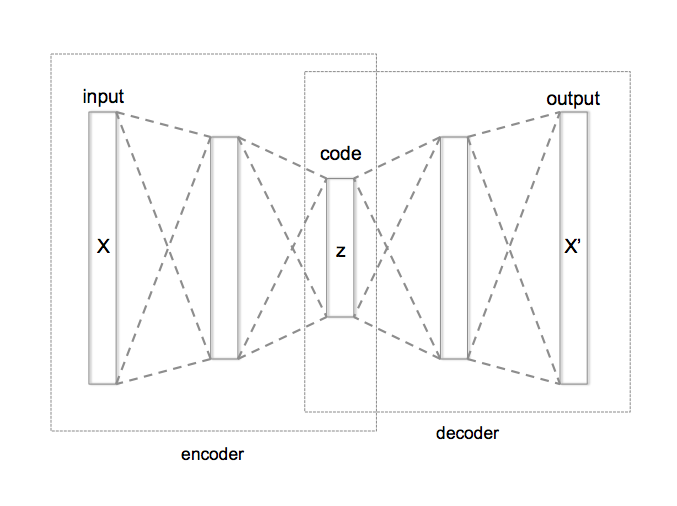
\includegraphics[width=.8\textwidth]{images/autoencoder-structure}
	\caption{\label{fig:autoencoder-structure} Schematic picture of an autoencoder architecture}
\end{figure}

By training a model to do this, two objectives can be achieved simultaneously:
\begin{itemize}
	\item The encoder part of the model could be used extract the most salient features of the data in a compressed representation, which is a friendlier format for downstream processing or learning algorithms. \citep{hinton2006reducing}
	\item The decoder part of the model could be used as a generator. Given that we can sample from the distribution of the existing latent representations learnt, or from a pre-defined prior (in a variational autoencoder), we can generate plausible novel data.
\end{itemize}

In the context of natural language the encoder can be utilized as a sentence-encoding feature-extractor and the decoder can be utilized as a generative model. Autoencoders are also used for being able to de-noise data given pairs of noisy and regular data, by learning a de-noising function. These properties in general make autoencoders a good framework to implement sequence-to-sequence models with.
